%%%%%%%%% Part II %%%%%%%%%

\par \noindent The following takes you through the steps of solving a simple general equilibrium model
that generates an endogenous steady state wealth distribution:\newline

\par\noindent \colorbox{black!12}{\textbf{Step 1.}}  We first take a price of discount bonds
$q \in [0,1]$ as given (assume that $\beta < q \leq 1$), then solve
the agent's dynamic programming problem for her decision rule $a'= g(a,s; q)$.
Define the operator $T$ on the space of bounded functions on $A \times S$
(bounded by virtue of the fact that $A \times \mathcal{S}$ is compact) by
\begin{eqnarray}
    (Tv)(a,s;q)
    = \max_{(c,a') \in \Gamma(a,s;q)} \left\{ u(c)
    + \beta \displaystyle{\sum_{s' \in \mathcal{S}} \Pi(s'|s)\, v(a',s';q)} \right\},
\end{eqnarray}
where
\begin{eqnarray}
    \Gamma(a,s;q) = \{ (c,a') \in \mathbb{R}_+ \times A : c + qa' \leq s + a \}
\end{eqnarray} is the set of feasible consumption-asset choices given state $(a,s)$ and bond price $q$.
Essentially, we solve for the value and policy functions given $q$ in this step.     \newline

\par\noindent \colorbox{black!12}{\textbf{Step 2.}} Given the decision rule $a' = g(a,s;q)$ in \textbf{Step 1.},
we next compute the invariant structure of wealth distribution. So, we take the decision rule $g_q$ as given,
define the operator $T^*$ on the space of probability measures $\Lambda(\tilde{A}\times \mathcal{S})$ by
\begin{eqnarray}
    (T^* \mu)(\tilde{A}_0, S_0)
    = \sum_{(a',s') \in \tilde{A}_0 \times S_0}
    \left\{ \sum_{(a,s) \in \tilde{A} \times \mathcal{S}}
    \chi_{\{a' = g_q(a,s)\}} \, \Pi(s'|s)\,\mu_q(a,s) \right\}.
\end{eqnarray}
\noindent
Here, $\chi_{\{a' = g_q(a,s)\}}$ is an indicator function that picks out combinations of $(a,s)$
which map to a given $a'$, and $\tilde{A}_0 \times S_0 \subseteq \tilde{A} \times S$.
Starting with a guess for $\mu(a,s;q)$, call it $\mu^0$, use the operator $T^*$
to define mappings $T^{*n}$ where $T^{*1}\mu^0 = T^*\mu^0$, $T^{*2}\mu^0 = T^*(T^*\mu^0)$, etc.
Thus, in this step, we are computing the invariant distribution $\mu(a,s;q)$ as the fixed point of $T^*$. \newline

\par\noindent \colorbox{black!12}{\textbf{Step 3.}} Finally, we check whether the bond market clears.
Embed the functions associated with \textbf{Step 1.} and \textbf{2.} into a program to calculate the
excess demand or supply of assets. Specifically, given the invariant distribution
$\mu(a,s;q)$ from \textbf{Step 2.}, check whether the asset market clears at the bond
price $q$ we started with in \textbf{Step 1.}, that is,
\begin{eqnarray}
    \text{ED}(q) \equiv \int_{A,\mathcal{S}} g_q(a,s)\,\mu^*_q(da,ds) = 0.
\end{eqnarray} \begin{itemize}
    \item If $\text{ED}(q) = 0$, the market clears and we are done.
    \item If $\text{ED}(q) > 0$, we need a higher bond price to make saving less attractive (raise $q$), and
    \item If $\text{ED}(q) < 0$, we need a lower bond price to make borrowing less attractive (lower $q$).
\end{itemize} Repeat \textbf{Steps 1.} and \textbf{2.} until the bond
market clears. The equilibrium bond price is then denoted by $q^{**}$.

\begin{remark} Here is an overview of the main functions in my \colorbox{blue!12}{\texttt{2 functions.jl}} file:
    \begin{itemize}
        \item[\circled{1}] \verb|Solve_HH(prim, res)| $\rightarrow$ Solves $T$ operator for given $q$
        \item[\circled{2}] \verb|Solve_Invariant(prim, res)| $\rightarrow$ Solves $T^*$ operator for distribution
        \item[\circled{3}] \verb|Update_q(res, tol)| $\rightarrow$ Checks market clearing and updates $q$
    \end{itemize} For asset space, I choose $A = [-2, 2.5]$ with 1000 grid points, where $2.5$ aligns with
    the upper bound in Dean's slides. And, I guess an initial bond price to be $q_0 = \beta + (1-\beta)/8$,
    which is artificially higher than the complete market benchmark $q = \beta$.
\end{remark}

\newpage

% Exercise 2.1
\begin{framedexercise}[Policy function $g(a,s)$]
    Plot the policy function $g(a,s)$ over $a$ for each $s$ to verify that there
    exists $\hat{a}$ where $g(\hat{a},s) < \hat{a}$ as in \textit{Figure 1 of Huggett}.
    (Recall this condition establishes an upper bound on the set $A$ necessary to
    obtain an invariant distribution).
\end{framedexercise}

\begin{solution} In Figure \ref{fig:policy}, I plot the policy function $g(a,s)$ over $a$ for each employment state $s$.
    There exists $\hat{a}$ where $g(\hat{a},s) < \hat{a}$ for both employed and unemployed states.
    Specifically, the thresholds are $\hat{a}_{\text{employed}} = 1.1261$ and $\hat{a}_{\text{unemployed}} = -2.0$ (in dashed lines).
    \begin{figure}[H]
        \centering
        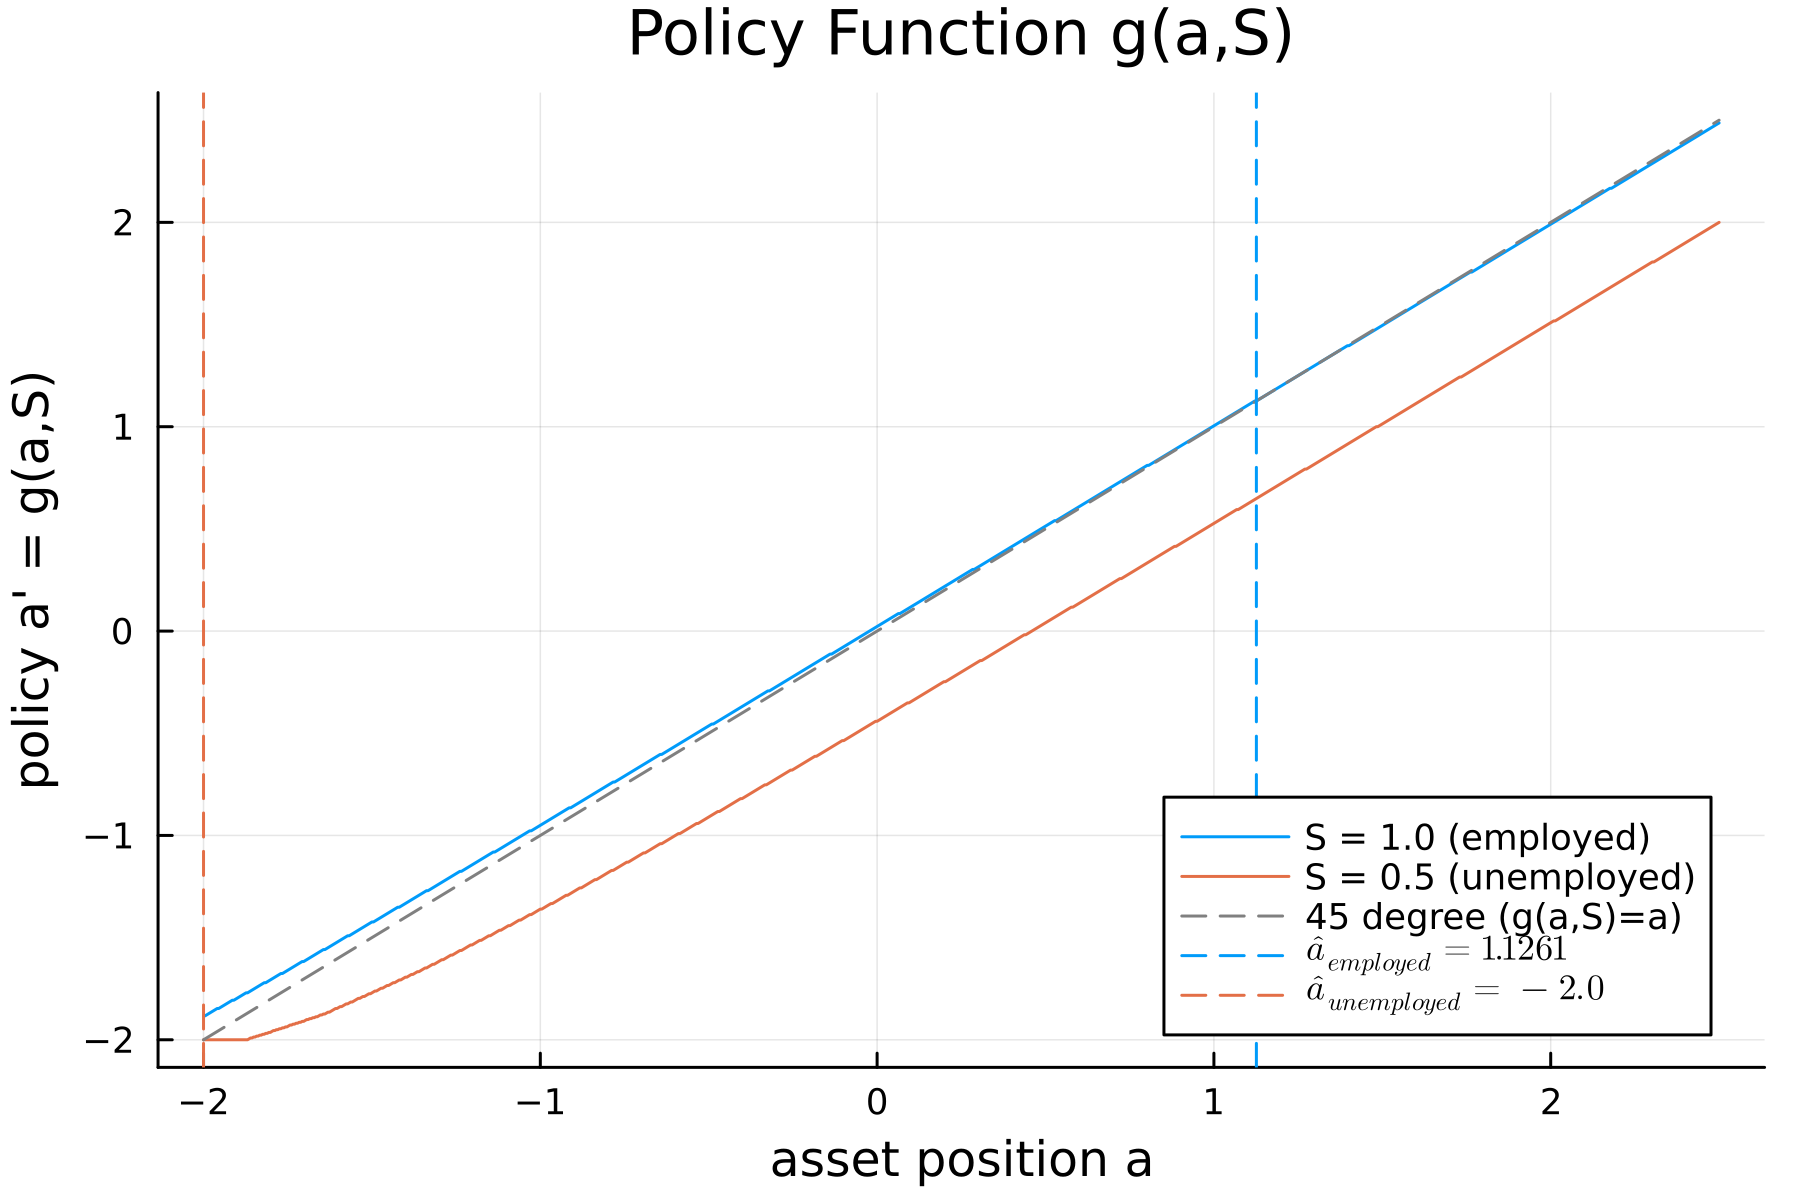
\includegraphics[width=0.85\textwidth, angle=0]
        {2 Policy_Functions.png}
        \caption{Policy Function}
        \label{fig:policy}
    \end{figure}
    \begin{remark}
        The employed agents should save, and the unemployed agents should dissave (i.e., borrow). \qed
    \end{remark}
\end{solution}

\newpage
% Exercise 2.2
\begin{framedexercise}[Equilibrium bond price $q^{**}$] What is the equilibrium bond price?
    Plot the cross-sectional distribution of wealth for
    those employed and those unemployed on the same graph.
\end{framedexercise}

\begin{solution}
    In this incomplete market, the equilibrium price of bonds is $q^{**} = 0.9942462299971491 \approx 0.99425$
    (slightly higher than complete market benchmark $q = \beta$). The cross-sectional distribution of wealth for
    those employed and those unemployed is plotted in Figure \ref{fig:wealth}.
    \begin{figure}[H]
        \centering
        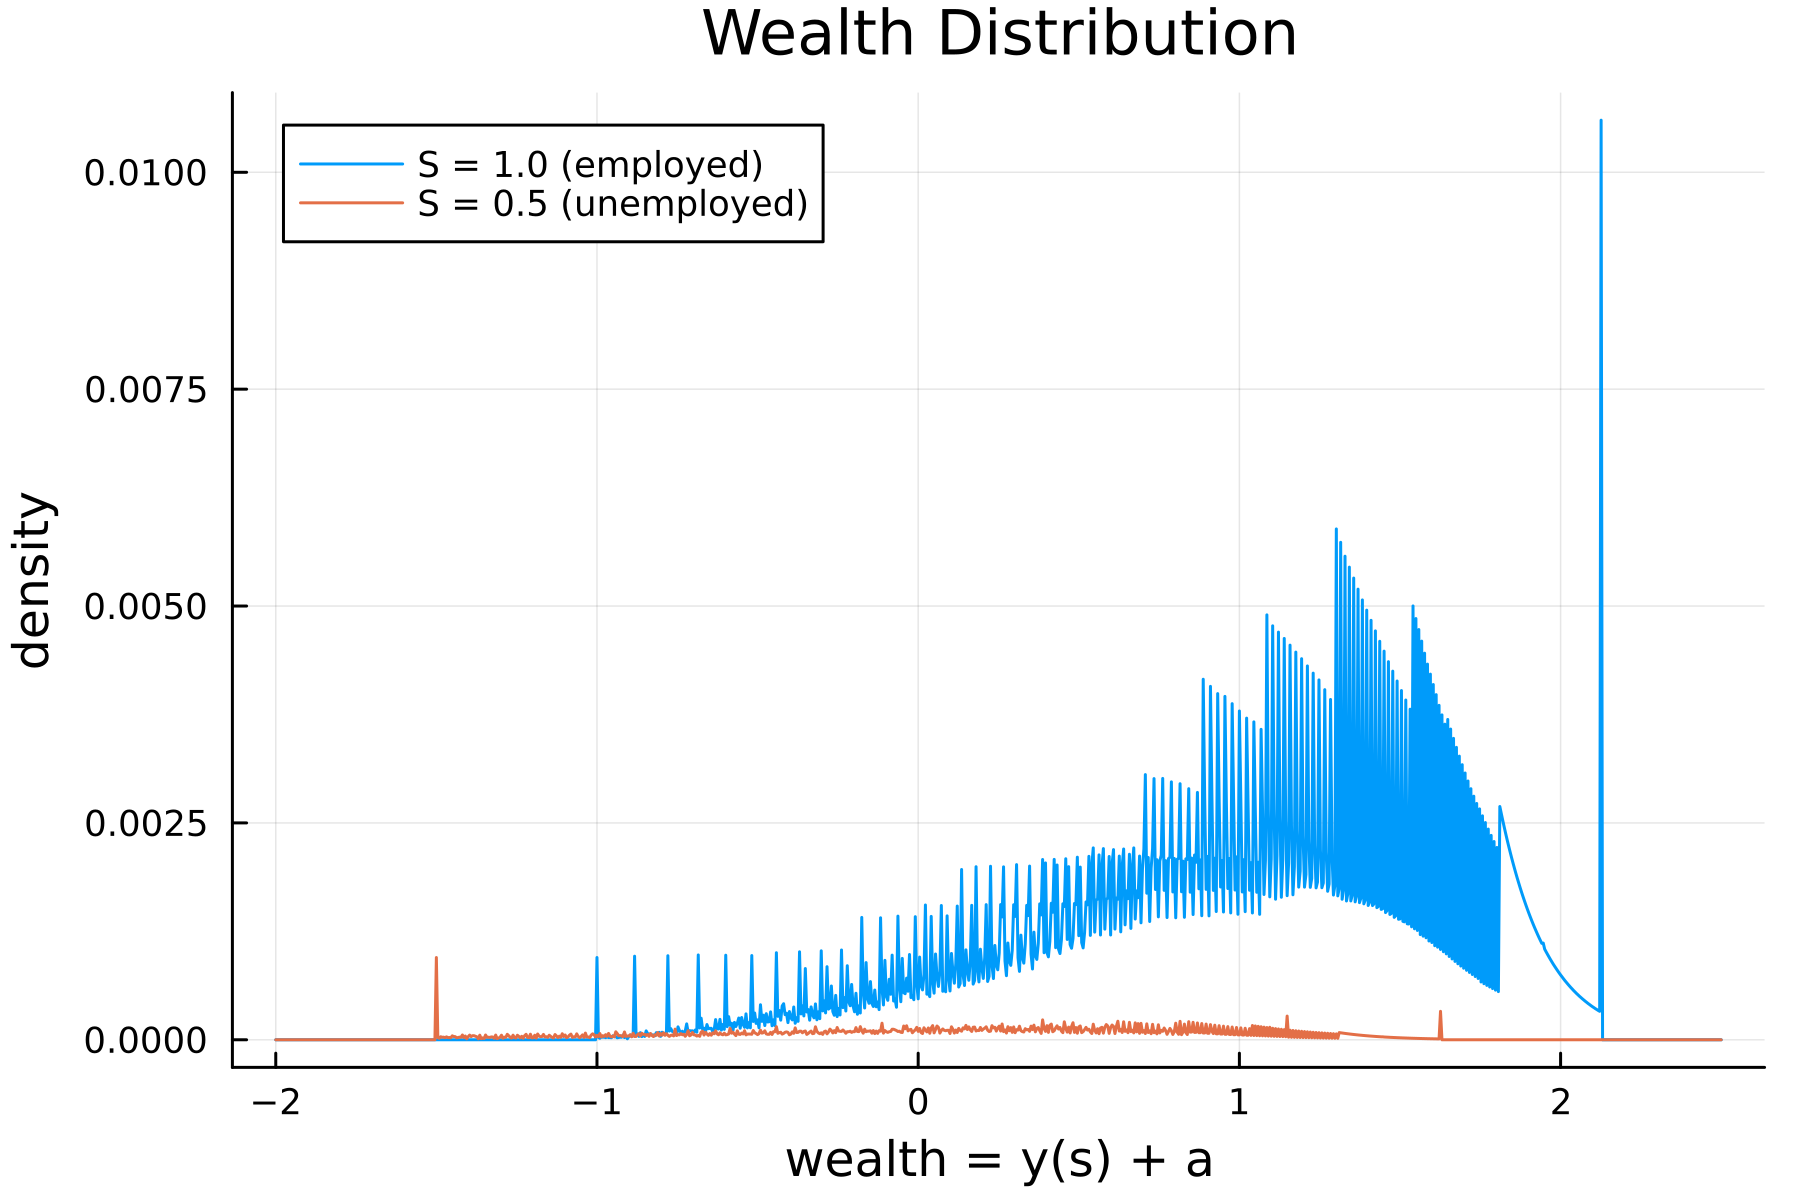
\includegraphics[width=0.85\textwidth, angle=0]
        {3 Wealth_Distributions.png}
        \caption{Wealth Distribution}
        \label{fig:wealth}
    \end{figure}
    \begin{remark}
        The wealth of employed agents peak at $2.1261$
        and that of unemployed peak at $-1.5$. In general, the employed agents hold more wealth
        than the unemployed agents, as expected. \qed
    \end{remark}
\end{solution}

\newpage
% Exercise 2.3
\begin{framedexercise}[Lorenz curve and Gini coefficient]
    Plot a Lorenz curve.What is the gini index for your economy? Compare
    them to the data. For this problem set, define wealth as current earnings (think
    of this as direct deposited into your bank, so it is your cash holdings) plus net
    assets. Since market clearing implies aggregate assets equal zero, this wealth
    definition avoids division by zero in computing the Gini and Lorenz curve
\end{framedexercise}

\begin{solution}
    My calculated Gini coefficient is $0.38525$, which is not too far from the ballpark of empirical estimates
    of wealth inequality in the U.S. (between $0.4$ and $0.5$ in year 2024). The Lorenz curve is plotted in Figure \ref{fig:lorenz}.
    \begin{figure}[H]
        \centering
        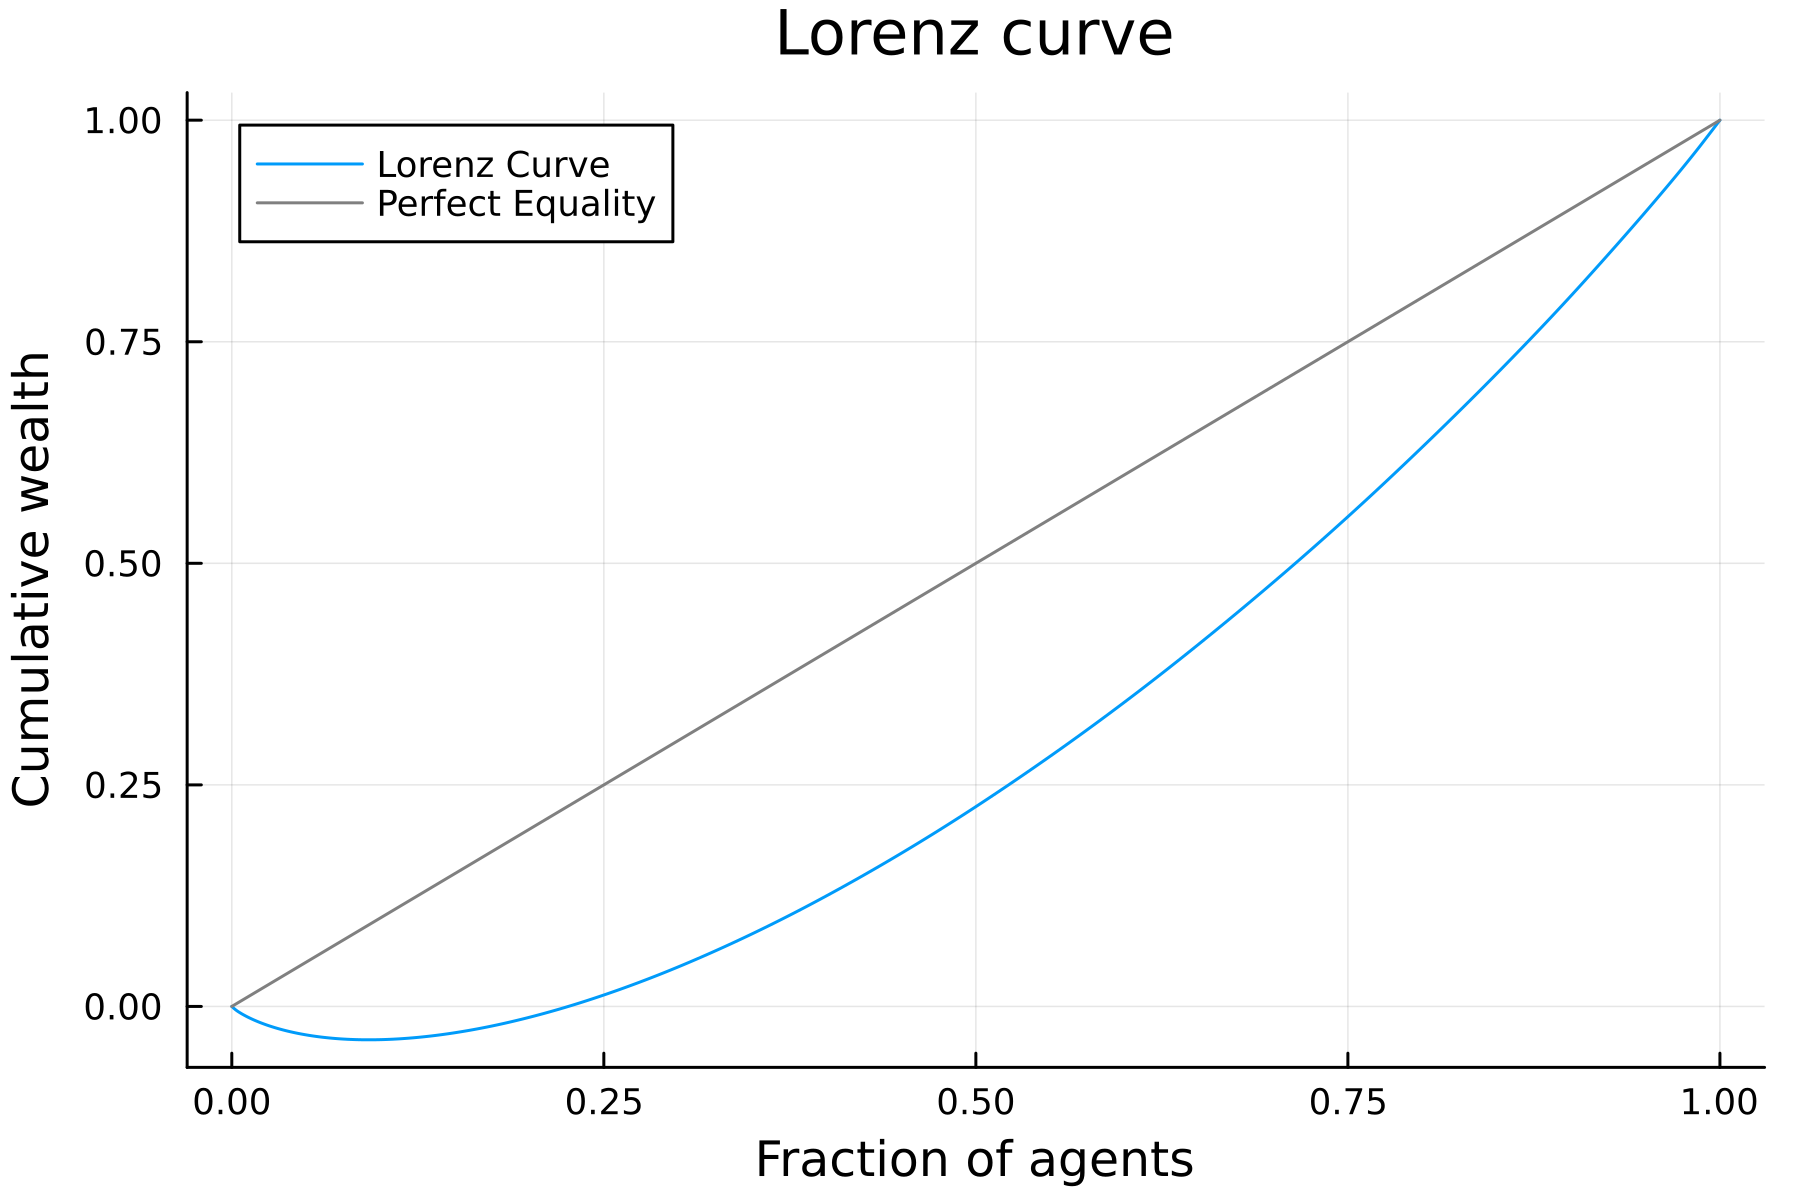
\includegraphics[width=0.85\textwidth, angle=0]
        {4 Lorenz_Curve.png}
        \caption{Lorenz Curve}
        \label{fig:lorenz}
    \end{figure}
    \begin{remark}
        The Lorenz curve is negative in the
        first quantile because, in the model, the sum of the wealth of agents in that quantile is less than zero. \qed
    \end{remark}
\end{solution}






% Here is my output from Julia terminal:

\begin{comment}
=============================================
Huggett model with 2 employment states, 1000 asset grid points
=============================================
ED is within tolerance, with: 1.1538807858983008e-5
-> Bond price converges to: 0.9942462299971491
-> Asset/bond Market clears!

Market clears in 50 iterations

=============================================

Time: 44.834 seconds to solve this Huggett model (tol level = 10^-4).

=== STATIONARY DISTRIBUTION (2×2, by Detailed Balance Equations) ===
Π₁₂ (employed → unemployed): 0.03
Π₂₁ (unemployed → employed): 0.5
π[employed] = π₂₁/(π₁₂+π₂₁) = 0.5/0.53 = 0.9434
π[unemployed] = π₁₂/(π₁₂+π₂₁) = 0.03/0.53 = 0.0566
Sum (should be 1.0): 0.9999999999999999
Verification π*Π ≈ π: true
==============================================

=== POLICY FUNCTION ===
Threshold asset levels where g(a,s) = a:
a*_employed = 1.1261
a*_unemployed = -2.0

=== WEALTH DISTRIBUTION ===
Total mass in wealth distribution: 0.9999999999999247
Max density - Employed: 0.01060043773137361
Max density - Unemployed: 0.0009482107314441653
Employed peak at wealth level: 2.126126126126126
Unemployed peak at wealth level: -1.5

=== LORENZ CURVE AND GINI COEFFICIENT ===
=== GINI CALCULATION ===
Area under Lorenz curve: 0.30737436669923607
Gini coefficient: 0.38525126660152786
Rounded to 5 digits: 0.38525.
Expected range: [0, 1] where 0=perfect equality, 1=perfect inequality
===================================

=== Welfare in complete markets (First Best) ===
w_FB (rounded to 5 digits): -4.25252.

=== Welfare in incomplete markets (Counterfactual) ===
w_inc (rounded to 5 digits): -4.45153.
REMARK: This alignes to class slides,
'Aggregate welfare is higher in the complete markets economy than
the incomplete markets economy (no surprise)'.


Welfare gain of switching to complete markets (rounded to 5 digits): 0.00134.
Fraction of agents that favor switching to complete markets (rounded to 5 digits): 0.54145.
\end{comment}